\documentclass{article}

\usepackage{array}
\usepackage{amsfonts}
\usepackage{amsmath}
\usepackage{geometry}
\usepackage{stmaryrd}
\usepackage{pgfplots}
\usepackage{rotating}


\geometry{hmargin=2.5cm,vmargin=1.5cm}
\title{IEOR 262 : Homework 3}
\author{Arnaud Minondo}

\begin{document}
\maketitle
\section*{Problem 1.16 :}
Let $p_1,p_2,p_3$ the number of time process 1, 2, 3 are processed.
The problem is : $$\boxed{\max(200p_1+60p_2+206p_3) \text{ s.t. }\begin{array}{c}
    3p_1+p_2+5p_3 \leq 8*10^6 \\
    5p_1+p_2+3p_3\leq 5*10^6 \\
    p_1,p_2,p_3 \ge 0 \\
\end{array} }$$

\section*{Problem 1.17 :}
Let $\forall i \in\llbracket 1;n\rrbracket, x_i$ be the fraction of $s_i$ sold.
The problem is : $$\boxed{\max\left(\sum\limits_{i=1}^n r_is_i(1-x_i)\right) \text{ s.t. } \begin{array}{c}
    \sum\limits_{i=1}^n{x_is_ip_i} \ge K\\
    \forall i \in \llbracket 1;n\rrbracket, 0\leq x_i\leq 1\\
    
\end{array}}$$
\section*{Problem 2.10 :}
\subsection*{(a)}
If $n = m+1$ then we can define : $\forall i \in \llbracket 1;m \rrbracket, P_i = (x\in\mathbb{R}^n| a_i x = b_i)$ where $a_i$ is the $i$-th row of $A$ and $b_i$ is the $i$-th coefficient of b.
\\
We can notice that $P = \cap_{i=1}^m P_i$ where $P_i$ is a hyperplane
 of $\mathbb{R}^n$ and you have $\dim(P_i) = n-1$. Each $a_i$ is perpendicular
 to $P_i$, and as each $a_i$ are linearly independent the intersection of two
 hyperplanes will reduce the dimension of at least 1. So we have $\dim(P) = \dim(\cap_{i=1}^mP_i)\leq n-m = 1$.
 There can only be two extreme points on a line.
\subsection*{(b)}
I will only consider the case where $P$ is nonempty and related to a linear optimization problem that is bounded.
 In this case : an optimal solution is a basic point and there is only a
 finite number of basic points as there are only m constraints so at most $\binom{n}{m}$ basic points. As it is a finite set it is bounded.
\subsection*{(c)}
This is false : let $(\mathcal{P})$ : $\min(x_1-x_2)$ s.t. $x_1-x2 = 1$, $x_1,x_2 \ge 0$, then $x_1 = \frac{3}{2}, x_2 = \frac{1}{2}$ is optimal but not basic and more than 1 variable is non zero.
\subsection*{(d)}
This is true : let $x_1, x_2\in P$ be two optimal solution, let $\lambda\in [0;1]$ and $x_\lambda = \lambda x_1 + (1- \lambda)x_2 \ge 0$ then $ Ax_\lambda = \lambda Ax_1 + (1- \lambda)Ax_2 = b$ thus $x_\lambda\in P$ and $c^Tx_\lambda = \lambda c^Tx_1 + (1- \lambda)c^Tx_2 = c^Tx_1$ which is the optimal value.
Therefore there are infinetely many optimal solutions.
\subsection*{(e)}
This is false : let $(\mathcal{P})$ : $\min(x1-x2)$ s.t. $x_1-x_2 = 0$ , $x_1\ge 0, x_2\ge 0$. There are multiple optimal solutions but only one basic optimal solution.
\subsection*{(f)}
Let $P=\{(x_1,x_2,x_3)\in\mathbb{R}^n | x_1+x_2+x_3 = 1\}$ and $(\mathcal{P})$ : $\min(\max(x_1-x_2+x_3,-x_1+x_2-x_3))$ s.t. $x_1,x_2,x_3\in P$ then an optimal solution is $x_1 = \frac{1}{2}, x_2 = \frac{1}{2},x_3 = 0$ and is not a basic solution as only two constraints are active.

\section*{Problem 3.12 :}
\subsection*{(a)}
The problem in standard form is  : $$\boxed{\min(-2x_1-x_2) \text{ s.t. } \begin{array}{c}
    x_1-x_2+s_1 = 2\\
    x_1+x_2+s_2 = 6\\
    x_1,x_2,s_1,s_2\ge 0
\end{array}}$$
A solution to this problem would be $x_1 = 0,x_2 = 0, s_1 = 2, s_2 = 6$
\subsection*{(b)}
Starting from the point : $(x_1,x_2,s_1,s_2) = (0, 0, 2, 6)$.
\\\\
$
\begin{array}{|c|cccc|}
    \hline
    0& -2&-1&0&0\\
    \hline
    2&1 & -1& 1&0\\
    6&1&1&0&1\\
    \hline
\end{array}$\\
$x_1$ and $x_2$ reduced cost are both negative so I will choose that $x_1$ enters the basis, we compute $\theta = 2$ and $s_1$ leaves the basis.
\\\\
The new array is :
$
\begin{array}{|c|cccc|}
    \hline
    4& 0&-3&2&0\\
    \hline
    2&1 & -1& 1&0\\
    4&0&2&-1&1\\
    \hline
\end{array}$
\\
$x_2$ reduced cost is negative so $x_2$ enters the basis. Compute $\theta = 2$ and $s_2$ leaves the basis.
\\\\
The new array is :
$\begin{array}{|c|cccc|}
    \hline
    10&0&0&0.5&1.5\\
    \hline
    4&1&0&0.5&0.5\\
    2&0&1&-0.5&0.5\\
    \hline
\end{array}$
\\
No reduced costs are negative so the point $\boxed{x_1=4,x_2=2,s_1=0,s_2=0}$ is optimal.
\\
\subsection*{(c)}
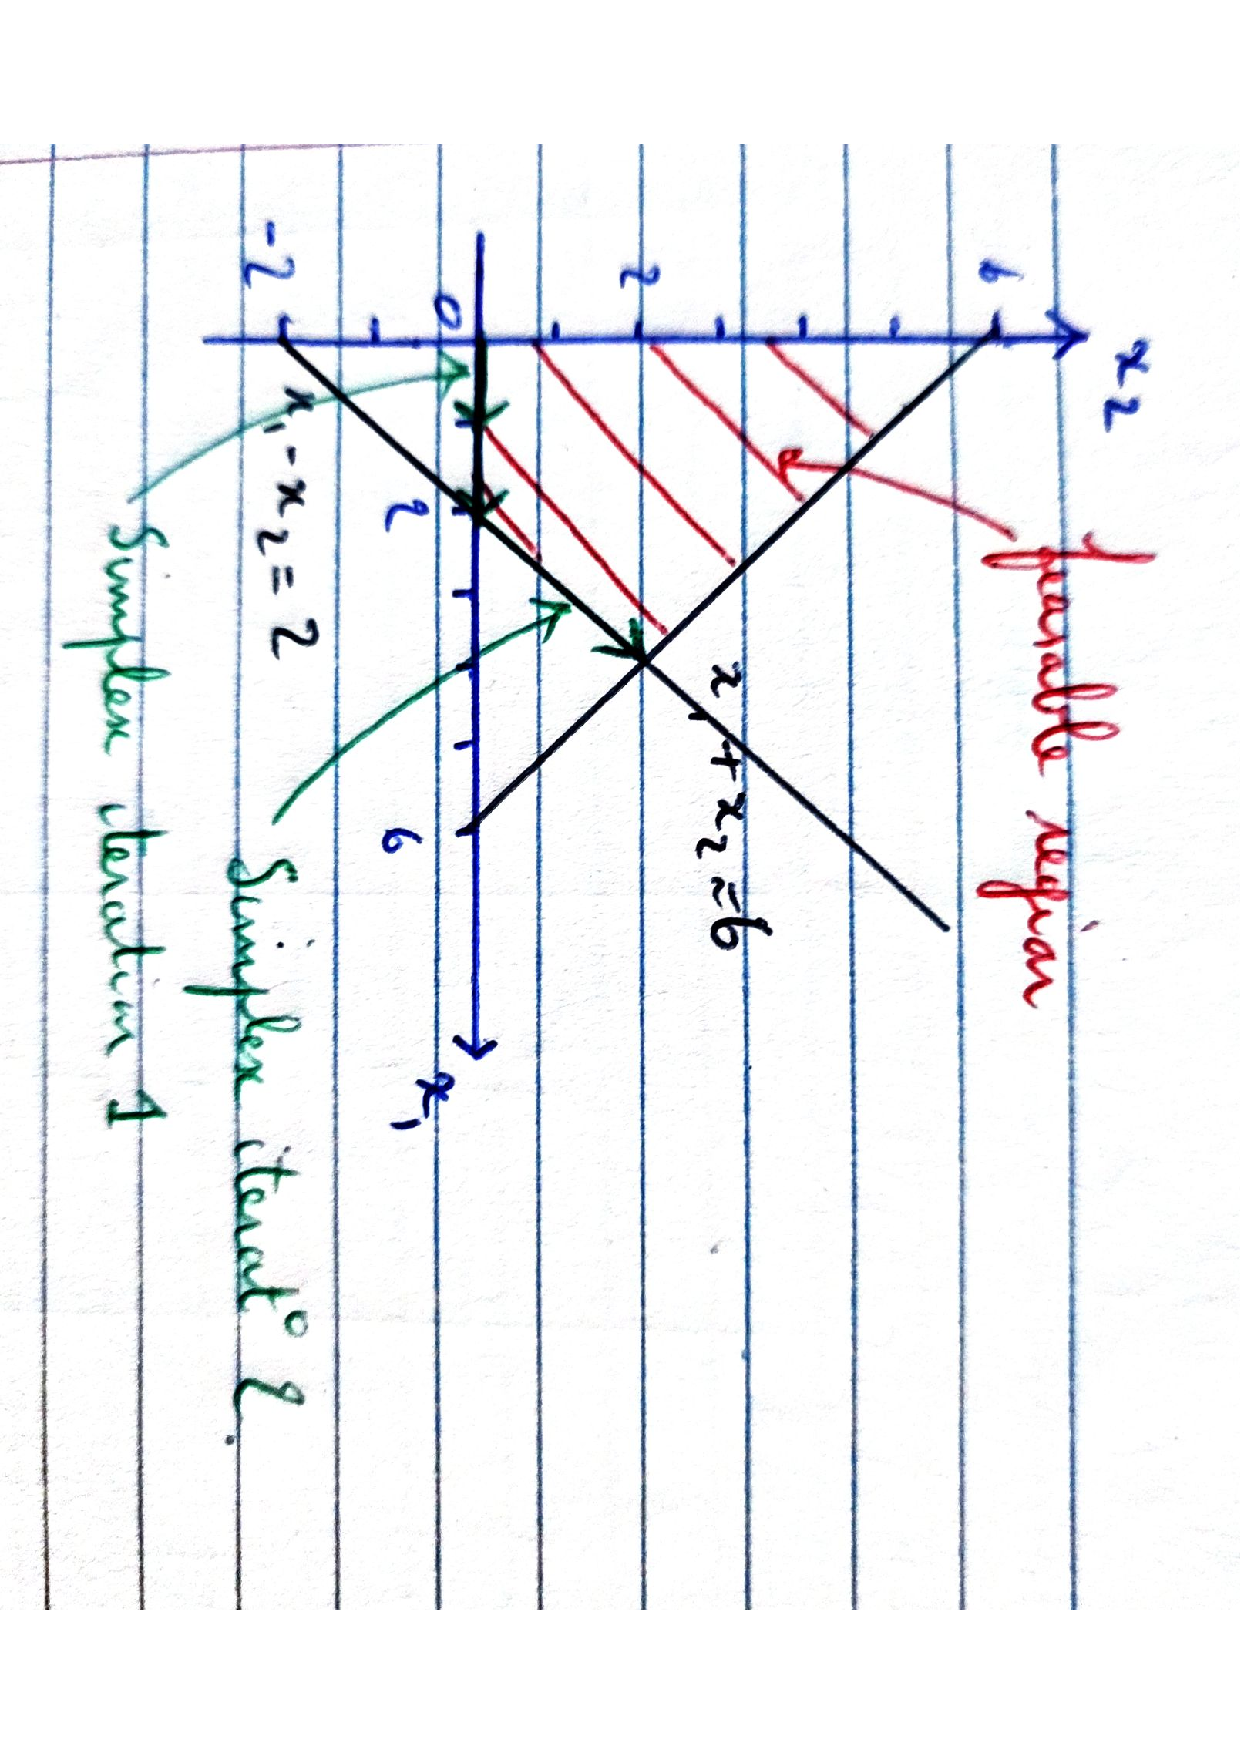
\includegraphics[width = 0.4\textwidth, height =0.6\textwidth, angle = 90]{img/Document 3.pdf}
\newpage
\section*{Problem 3.17 :}
The phase I :\\
Intialisation : as $B = I_3$, the reduced cost vector $\overline{c_N} = (0,0,0,0,0) - (1,1,1)N$ where $N = \left(\begin{array}{ccccc}
    1&3&0&4&1\\
    1&2&0&-3&1\\
    -1&-4&3&0&0\\
\end{array}\right)$, 
$\begin{array}{|c|ccccc|ccc|}
    \hline
    5&-1 &-1&-3&-1&0&0&0&0\\
    \hline
    2 & 1&3&0&4&1&1&0&0\\
    2& 1 & 2 &0 &-3 &1 &0 &1 &0\\
    1 &-1&-4&3&0&0&0&0&1\\
    \hline
\end{array}$ $x_1$ enters the basis and $s_1$ leaves gives the new array :
\\\\\\
 $\begin{array}{|c|cccccccc|}
    \hline
    3 & 0&2&-3&3&0&1&0&0\\
    \hline
    2&1&3&0&4&1&1&0&0\\
    0&0&-1&0&-7&0&-1&1&0\\
    3&0&-1&3&4&1&1&0&1\\
    \hline
\end{array}$ $x_3$ enters the basis and $s_3$ leaves gives the new reduced cost vector : $\overline{c_N} = (1,7,1,2,1)\ge 0$ so the solution $x_1 = 2, x_3=1$ and the others equal to 0 is optimal. But as $s_2$ is still in the basis we apply a change of basis : $s_2$ leaves and $x_2$ enters.
\\
The final tableau is :
$\begin{array}{|c|cccccccc|}
    \hline
    3 & 0&2&-3&3&0&1&0&0\\
    \hline
    2&1&0&0&-17&1&-2&3&0\\
    0&0&1&0&7&0&1&-1&0\\
    1&0&0&3&11&1&2&-1&1\\
    \hline
\end{array}$
\\\\
Phase II :
\\
Taking $x_1,x_2,x_3$ as the basis, $B = \left(\begin{array}{ccc}
    1&3&0\\
    1&2&0\\
    -1&-4&3\\
\end{array}\right)$ and $B^{-1} = \left(\begin{array}{ccc}
    -2&3&0\\
    1&-1&0\\
    2/3&-1/3&1/3\\
\end{array}\right)$, reduced cost vector is (3,-5) and the array is 
$\begin{array}{|c|ccccc|}
    \hline
    7&0&0&0&3&-5\\
    \hline
    2&1&0&0&-17&1\\
    0&0&1&0&7&0\\
    1&0&0&1&11/3&1/3\\
    \hline
\end{array}$. Thus $x_5$ enters the basis and $x_1$ leaves and the new array is 
$\begin{array}{|c|ccccc|}
    \hline
    -1&5&0&0&-82&0\\
    \hline
    2&1&0&0&-17&1\\
    0&0&1&0&7&0\\
    1/3&-1/3&0&1&28/3&0\\
    \hline
\end{array}$ and $\boxed{x_5=2,x_3=1/3\text{ is an optimal degenerate solution of the pb}}$ as $x_4$ has to enter the base but $x_2 = 0$ has to leave the basis and you are going to exchange forever those two.

\section*{Problem 3.19 :}
\subsection*{(a)}
Let $\alpha = 0,\beta = 0, \gamma = 0,\eta= 0, \delta=-2$, there are mulitple solutions.
\subsection*{(b)}
Let $\alpha = -1,\gamma = -1, \beta = 1,\eta = 1,\delta = -1$ the problem is unbounded as if $x_1$ is chosen to enter the basis then all coefficient are negative and you can choose any $\theta$.
\subsection*{(c)}
Let $\alpha = 1, \gamma = 1, \beta = 1,\eta = 1,\delta = -1$.

\section*{Problem 4.33 :}
Let $p_S = S$ be the price of the stock, $p_B = 1$ the price of the bond and $p_O$ the price of the option.
$R = \left(\begin{array}{ccc}
    Su& r& \max(0,Su-K)\\
    Sd& r& \max(0,Sd-K)\\
\end{array}\right)$, after theorem 4.8, the absence of arbitrage condition yields there exist $\delta,\gamma>=0$ such that $p_S = \gamma Su + \delta Sd = S$ and $p_B = \gamma r + \delta r$ and $p_O = \gamma \max(0,Su-K)+\delta \max(0,Sd-K)$
\\
So : $$\boxed{p_O = \gamma \max(0,Su-K)+\delta \max(0,Sd-K)\text{ where }1 =\gamma u +\delta d \text{ and }\frac{1}{r} = \delta +\gamma}$$
\section*{Problem 4.39 :}
Let $A \in \mathcal{M}_{m,n}(\mathbb{R})$ without any loss of generality suppose n rows of $A$ are linearly independent. We can suppose this because if there exist an dependent row we can drop it. Let $C =\{x\in\mathbb{R}^n| Ax\ge 0\}$.
\\\\
\textbf{Definition 1 :} $d\in C$ is an extreme ray if there are n-1 constraints bounding.
\\
\textbf{Definition 2 :} $d\in C$ is an extreme ray if $\forall (f,g)\in C^2, f+g = d \implies (f,g)\in \text{Vect}(d)^2$
\\\\
Suppose $d\in C$ extreme ray after definition 1 ie. $\forall i\in\llbracket 1;n-1\rrbracket, \sum\limits_{j=1}^n a_{ij}d_j = 0$.
\\
Let $f,g\in C$ such that $d=f+g$, if $f =0 or g = 0$ then either $f=d$ or $g=d$ so we can suppose $f\neq 0$ and $g\neq 0$.
\\ 
Thus $\sum\limits_{j=1}^n a_{ij}f_{j} + \sum\limits_{j=1}^n a_{ij}g_{j} = 0$ (1)
\\
Moreover, $f\in C$ so $Af\ge 0$ so $\forall i \llbracket 1;m\rrbracket $, $\sum\limits_{j=1}^n a_{ij}f_j \ge 0$ and the same holds for g.
\\
Both terms in (1) are positive and the sum is equal to 0 thus both terms have to be 0.
\\
Thus $\forall i\in\llbracket 1;n-1\rrbracket$, $\sum\limits_{j=1}^n a_{ij}f_j = 0$ and $\sum\limits_{j=1}^n a_{ij}g_j = 0$.
\\
Now suppose that $f\notin \text{Vect}(g)$ then $\dim(\text{Vect}(f,g)) = 2$  and $\text{Vect}(f,g)$ is orthogonal to $\text{Vect}(a_1,a_2,a_3,...,a_{n-1})$.
\\
By learly independence hypothesis : $\dim(\text{Vect}(a_1,...,a_{n-1})) = n-1$ 
\\
Thus $\dim(\text{Vect}(a_1,a_2,...,a_{n-1})+\text{Vect}(f,g)) = n+1$ but $\text{Vect}(a_1,a_2,...,a_{n-1})+\text{Vect}(f,g)\subseteq\mathbb{R}^n$ and we have a contradiction.
\\
So $f$ is proportional to $g$ ie. $\exists \lambda\in\mathbb{R}^n$ s.t. $f = \lambda g$, moreover $A(\lambda g)\ge 0$ so $\lambda \ge 0$ thus $d = f+g = (1+\lambda) g = (1+\frac{1}{\lambda})f$ and both are proportional to $d$.
\\\\
Now let $d$ an extreme ray after definition 2 ie. $\forall (f,g)\in C^2, f+g = d \implies (f,g)\in \text{Vect}(d)^2$.
\\
Let $f$ be an extreme ray after definition 1 and $g = d-f$ we have $f = d - g$ and after proof 1 we have $d$ verifies n-1 bounds. 
\end{document}